\section{Opis szyfru\cite{4}}
% opis szyfru, jaka jest jego struktura, jakie prymitywy wykorzystuje, jakie parametry

SM4 to chiński standard szyfrowania blokowego, wprowadzony do ochrony sieci bezprzewodowych i wydany w styczniu 2006 roku. Wejście, wyjście i klucz SM4 mają 128 bitów.
Algorytm ma 32 rundy, z których każda modyfikuje jedno z czterech 32-bitowych słów. Szyfrowanie i
deszyfrowanie ma tę samą strukturę, z wyjątkiem tego, że klucz do deszyfrowania to
odwrotność klucza do szyfrowania.

\subsection{Definicje}

Następujące definicje są kluczowe do opisania struktury szyfru SM4.

\subsubsection{Słowo i bajt}

Zdefiniujmy $Z^{e}_{2}$ jako zbiór e-bitowych wektorów. Słowo wykorzystywane w algorytmie szyfrowania SM4 jest elementem $Z^{32}_{2}$, natomiast bajt elementem $Z^{8}_{2}$.

\subsubsection{S box}

S box, czyli blok podmiany (ang. substitution), przyjmuje 8 bitów na wejściu i zwraca 8 bitów na wyjściu. 

\subsubsection{Podstawowe operacje}

Podstawowymi operacjami bitowymi używanymi w omawianym algorytmie są:
\begin{enumerate}
    \item $\oplus$ --- bitowy XOR dwóch wektorów z $Z^{32}_{2}$
    \item $<<< \textit{i}$ --- obrót bitowy w lewo o \textit{i} bitów
\end{enumerate}

\subsubsection{Wejście, wyjście i klucz}

Tekst jawny to 128-bitowy blok składający się z czterech 32-bitowych słów $X = (X_0, X_1, X_2, X_3)$. Szyfrogram to analogiczny do tekstu jawnego 128-bitowy blok składający się z czterech 32-bitowych słów $Y = (Y_0, Y_1, Y_2, Y_3)$.

Klucz podawany do szyfru również zachowuje tę samą konwencję $MK = (MK_0, MK_1, MK_2, MK_3)$. Używany jest do generowania zestawu kluczy rund $(rk_0, rk_1, \ldots, rk_{31})$, gdzie $rk_i \in Z^{32}_2$.

\subsection{Funkcja rundy F}

Niech blok $(X_0, X_1, X_2, X_3) \in (Z^{32}_2)^4$ będzie 128-bitowym wejściem oraz $rk \in Z^{32}_2$ kluczem rundy, wówczas funkcja $F: (Z^{32}_2)^5 \rightarrow Z^{32}_2$:
\begin{equation*}
F(X_0, X_1, X_2, X_3, rk) = X_0 \oplus T(X_1 \oplus X_2 \oplus X_3 \oplus rk)
\end{equation*}

\begin{figure}[h!]
  \centering
  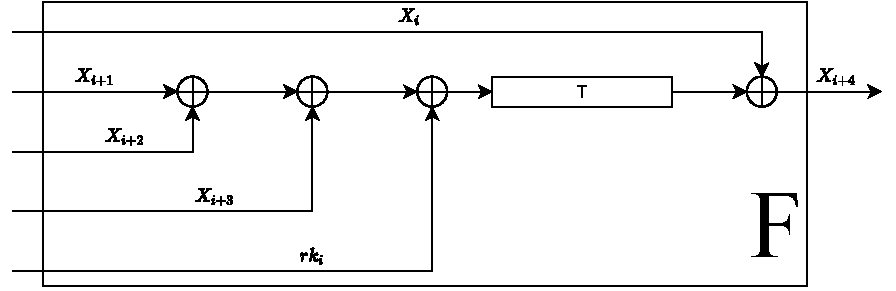
\includegraphics{diagramy/F.pdf}
  \caption{Blok F}
  \label{fig:F}
\end{figure}

\subsubsection{Mieszane podstawienie T}

$T: Z^{32}_2 \rightarrow Z^{32}_2$ jest odwracalną funkcją podstawienia. Składa się z nieliniowego podstawienia $\tau$ oraz liniowego  $L$.
\begin{equation*}
    T(\ldots) = L(\tau(\ldots))
\end{equation*}

\paragraph{Nieliniowe podstawienie $\tau$}\mbox{}

Niech $A$ będzie 32-bitowym słowem wejściowym, czyli $A = (a_0, a_1, a_2, a_3) \in (Z^8_2)^4$. Wówczas $\tau: (Z^8_2)^4 \rightarrow (Z^8_2)^4$ definiujemy następująco:

\begin{equation*}
    \tau(A) = (Sbox(a_0), Sbox(a_1), Sbox(a_2), Sbox(a_3))
\end{equation*}

\paragraph{Liniowe podstawienie $L$}\mbox{}

Niech B, będzie wynikiem otrzymanym z funkcji $\tau$. Wówczas funkcja $L: Z^{32}_2 \rightarrow Z^{32}_2$ definiowana jest następująco:

\begin{equation*}
    L(B) = B \oplus (B <<< 2)  \oplus (B <<< 10)  \oplus (B <<< 18)  \oplus (B <<< 24) 
\end{equation*}

\subsubsection{S box}

Działanie S boxa opisuje tabela \ref{table:sbox}. Wartości przedstawione są w systemie heksadecymalnym.

\begin{table}[h!]
\centering
\caption{S box}
\label{table:sbox}
\begin{tabular}{ | c | cccccccccccccccc | } 
\hline
 & 0 & 1 & 2 & 3 & 4 & 5 & 6 & 7 & 8 & 9 & a & b & c & d & e & f \\
\hline
0 & d6 & 90 & e9 & fe & cc & e1 & 3d & b7 & 16 & b6 & 14 & c2 & 28 & fb & 2c & 05 \\
1 & 2b & 67 & 9a & 76 & 2a & be & 04 & c3 & aa & 44 & 13 & 26 & 49 & 86 & 06 & 99 \\
2 & 9c & 42 & 50 & f4 & 91 & ef & 98 & 7a & 33 & 54 & 0b & 43 & ed & cf & ac & 62 \\
3 & e4 & b3 & 1c & a9 & c9 & 08 & e8 & 95 & 80 & df & 94 & fa & 75 & 8f & 3f & a6 \\
4 & 47 & 07 & a7 & fc & f3 & 73 & 17 & ba & 83 & 59 & 3c & 19 & e6 & 85 & 4f & a8 \\
5 & 68 & 6b & 81 & b2 & 71 & 64 & da & 8b & f8 & eb & 0f & 4b & 70 & 56 & 9d & 35 \\
6 & 1e & 24 & 0e & 5e & 63 & 58 & d1 & a2 & 25 & 22 & 7c & 3b & 01 & 21 & 78 & 87 \\
7 & d4 & 00 & 46 & 57 & 9f & d3 & 27 & 52 & 4c & 36 & 02 & e7 & a0 & c4 & c8 & 9e \\
8 & ea & bf & 8a & d2 & 40 & c7 & 38 & b5 & a3 & f7 & f2 & ce & f9 & 61 & 15 & a1 \\
9 & e0 & ae & 5d & a4 & 9b & 34 & 1a & 55 & ad & 93 & 32 & 30 & f5 & 8c & b1 & e3 \\
a & 1d & f6 & e2 & 2e & 82 & 66 & ca & 60 & c0 & 29 & 23 & ab & 0d & 53 & 4e & 6f \\
b & d5 & db & 37 & 45 & de & fd & 8e & 2f & 03 & ff & 6a & 72 & 6d & 6c & 5b & 51 \\
c & 8d & 1b & af & 92 & bb & dd & bc & 7f & 11 & d9 & 5c & 41 & 1f & 10 & 5a & d8 \\
d & 0a & c1 & 31 & 88 & a5 & cd & 7b & bd & 2d & 74 & d0 & 12 & b8 & e5 & b4 & b0 \\
e & 89 & 69 & 97 & 4a & 0c & 96 & 77 & 7e & 65 & b9 & f1 & 09 & c5 & 6e & c6 & 84 \\
f & 18 & f0 & 7d & ec & 3a & dc & 4d & 20 & 79 & ee & 5f & 3e & d7 & cb & 39 & 48 \\
\hline
\end{tabular}
\end{table}

Przykładowo dla wejścia '3f' odczytujemy 3-ci rząd i f-ą kolumnę: $Sbox('3f') = a6$. Sbox bazuje na operacji odwracania nad ciałem $GF(2^8)$ --- Ciało Galois.

\subsection{Kodowanie i dekodowanie}

Niech $R$ będzie odwrotnym podstawieniem:

\begin{equation*}
    R(A_0, A_1, A_2, A_3) = (A_3, A_2, A_1, A_0), A_i \in Z^{32}_2, i = 0, 1, 2, 3
\end{equation*}

Weźmy tekst jawny $(X_0, X_1, X_2, X_3) \in (Z^{32}_2)^4$, oznaczmy jego szyfrogram jako $(Y_0, Y_1, Y_2, Y_3) \in (Z^{32}_2)^4$. Załóżmy, że klucze poszczególnych rund zostały wygenerowane z klucza 128-bitowego i są definiowane jak następuje: $rk_i \in Z^{32}_2, i = 0,1, \ldots, 31$. Szczegóły generowania kluczy rund opisane są w sekcji \ref{section:roundKeys}.

Kodowanie przebiega w następujący sposób:

\begin{equation*}
    X_{i+4} = F(X_i, X_{i+1}, X_{i+2}, X_{i+3}, rk_i) = X_i \oplus T(X_{i+1} \oplus X_{i+2} \oplus X_{i+3} \oplus rk_i), i = 0,1,\ldots,31
\end{equation*}
        
\begin{equation*}
    (Y_0, Y_1, Y_2, Y_3) = R(X_{32}, X_{33}, X_{34}, X_{35})
\end{equation*}

Dekodowanie odbywa się za pomocą tego samego algorytmu, jedyną różnicą jest odwrotna kolejność kluczy rund. Klucze rund kodowania $(rk_0, rk_1, \ldots, rk_{31})$, klucze rund dekodowania $(rk_{31}, rk_{30}, \ldots, rk_0)$

\begin{figure}[H]
  \centering
  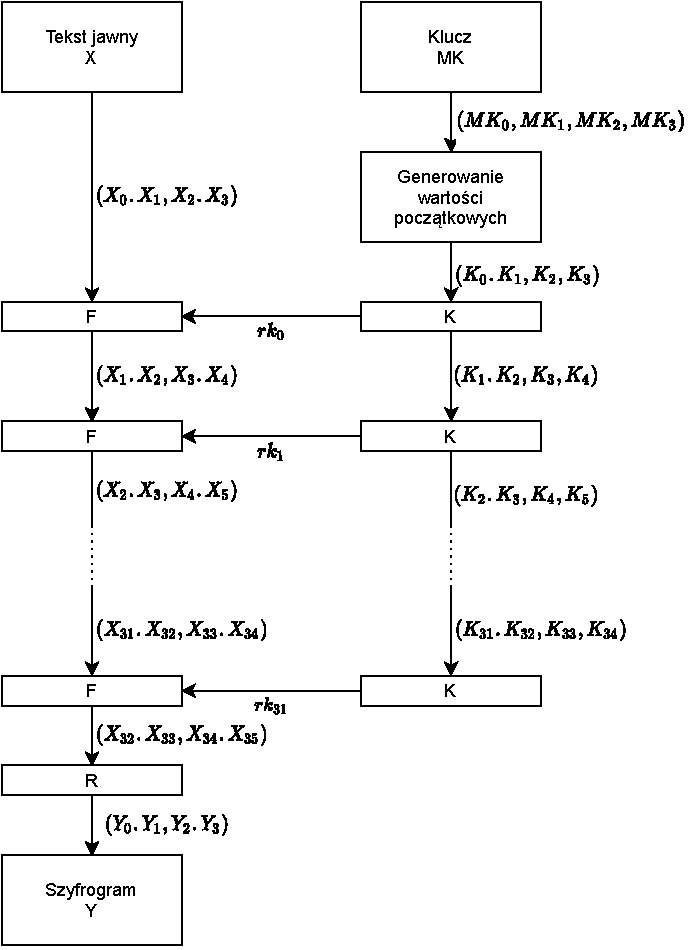
\includegraphics{diagramy/SM4.pdf}
  \caption{Schemat algorytmu szyfrowania SM4}
  \label{fig:SM4}
\end{figure}

Bloki F i K opisane są kolejno na Rysunku \ref{fig:F} i Rysunku \ref{fig:K}.

\subsection{Generowanie kluczy rund} \label{section:roundKeys}

Klucze rund generowane są z klucza 128-bitowego. Niech $MK = (MK_0, MK_1, MK_2, MK_3), MK_i \in Z^{32}_2, i = 0, 1, 2, 3$ będzie głównym kluczem 128-bitowym. Wówczas klucze rund $rk_i \in Z^{32}_2, i = 0, 1, \ldots, 31$ otrzymywane są w następujący sposób.
\begin{equation*}
    (K_0, K_1, K_2, K_3) = (MK_0 \oplus FK_0, MK_1 \oplus FK_1, MK_2 \oplus FK_2, MK_3 \oplus FK_3)
\end{equation*}

 Wówczas dla $i = 0, 1, \ldots, 31$:
\begin{equation*}
    rk_i = K_{i+1} = K_i \oplus T'(K_{i+1} \oplus K_{i+2} \oplus K_{i+3} \oplus CK_i)
\end{equation*}

\begin{figure}[H]
  \centering
  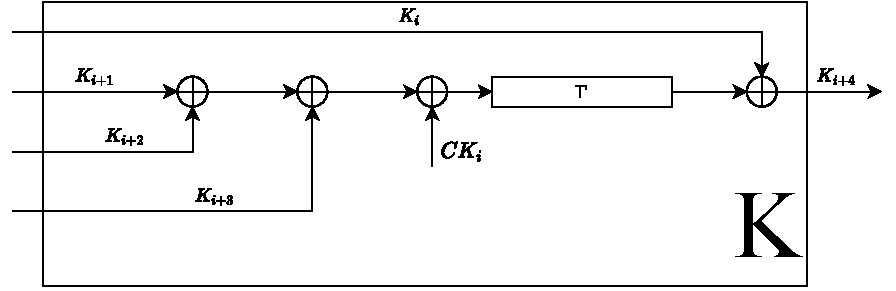
\includegraphics{diagramy/K.pdf}
  \caption{Blok K}
  \label{fig:K}
\end{figure}

\paragraph{Mieszane podstawienie T'}\mbox{}

Podstawienie T' jest defniowane tak samo jak podstawienie T z tą różnicą, że zamianst funkcji L używana jest następująca funkcja L':

\begin{equation*}
    L'(B) = B \oplus (B <<< 13) \oplus (B <<< 23)
\end{equation*}

\paragraph{Parametr FK}\mbox{}

Przytaczane parametry FK zdefiniowane są w notacji heksadecymalnej:

\begin{equation*}
    FK_0 = (a3b1bac6), FK_1 =  (56aa3350), FK_2 = (677d9197), FK_3 = (b27022dc)
\end{equation*}

\paragraph{Parametr CK}\mbox{}

Niech $ck_{i,j}$ będzie j-tym bajtem $CK_i = (ck_{i,0}, ck_{i,1}, ck_{i,2}, ck_{i,3}) \in (Z^8_2)^4$, gdzie $ck_{i,j} = (4i + j) \times 7 \pmod{256}$. Z tego wynika, że parametry CK są stałymi i nie ma potrzeby każdorazowego obliczania ich.








